{\begin{abstract}
本章では,Polylibプログラムのクラス構成,データ構造,入出力ファイルなどについて説明します.
\end{abstract}

% 
\graphicspath{{./fig_prg/}}

%
\section{クラス構成}

以下にPolylibのクラス図概要を示します.

\begin{figure}[H]
 \centering
 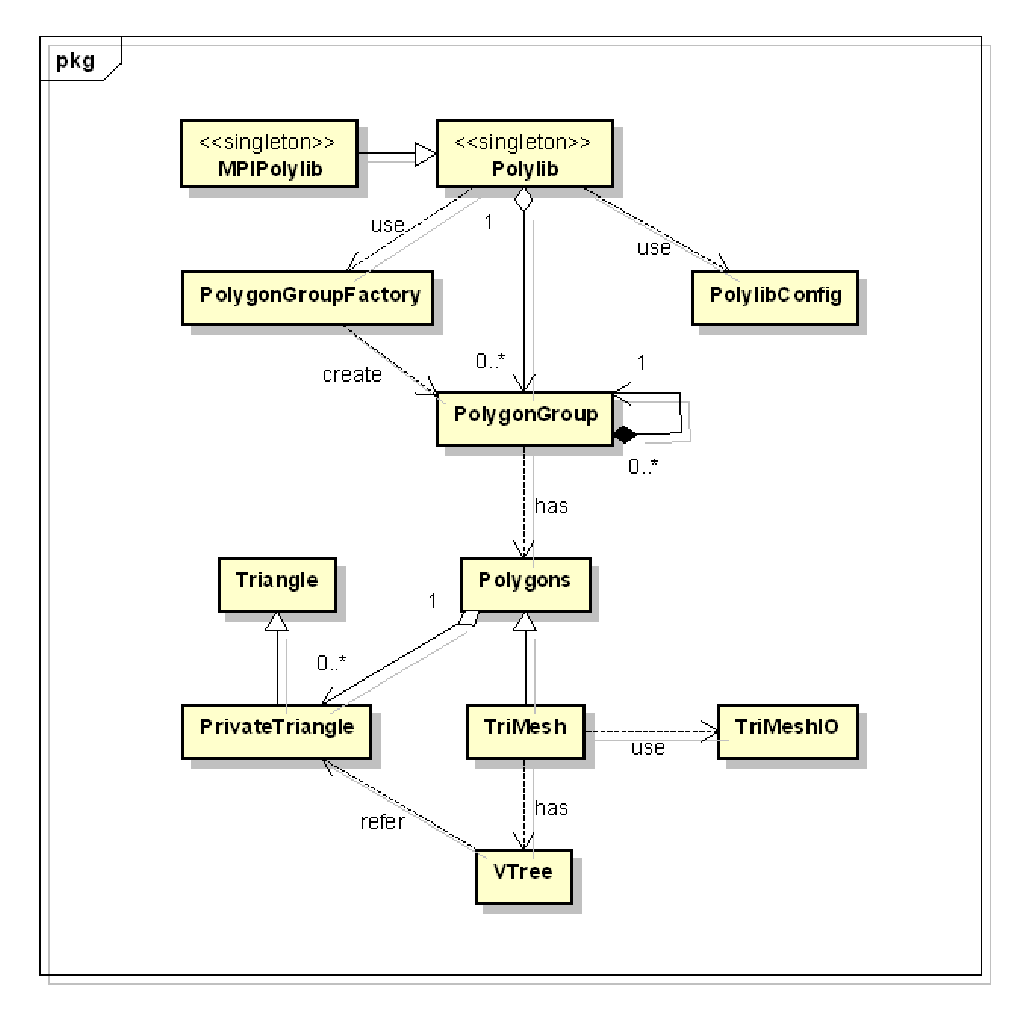
\includegraphics[width=12cm]{clip000.eps}
 \caption{主要クラス図}
\end{figure}

各クラスの説明は表\ref{tbl:classes}の通りです.

\pagebreak

\begin{table}[htbp]
 \begin{tabular}{|l|p{32em}|} \hline
 クラス名 & 概要 \\\hline
 \hline
 \multicolumn{1}{|l|}{Polylib} & 単一プロセス版のPolylib本体です.本クラス内部にポリゴングループ階層構造,三角形ポリゴン情報を保持します. \\
 \multicolumn{1}{|l|}{} & 本クラスはsingletonクラスであり,1プロセス内に1インスタンスのみ存在します. \\\hline
 MPIPolylib & MPI版のPolylib本体です.Polylibクラスを継承しており,各メソッドは並列処理を前提とした内容にオーバーライドされています. \\\hline
 PolylibConfig & Polylib初期化ファイルをload/saveするためのユーティリティクラスです. \\\hline
 PolygonGroup & 三角形ポリゴン集合をグルーピングして管理するためのクラスです.ポリゴングループ同士の階層的な包含関係も表現します.STLファイルから読み込んだ三角形ポリゴン集合を本クラスの属性であるPolygonsクラスインスタンスで管理します. \\\hline
 PolygonGroupFactory & Polylib初期化ファイルに記述されたポリゴングループ階層構造情報を元にPolygonGroupクラスとその継承クラスインスタンスを生成する処理を行うクラスです. \\\hline
 Polygons & 三角形ポリゴン情報を保持するコンテナクラスであり,ポリゴン検索のための検索メソッドを定義した抽象クラスです. \\\hline
 TriMesh & KD木による三角形ポリゴン検索アルゴリズムを実装したPolygonsクラスの導出クラスです. \\\hline
 TriMeshIO & STLファイルをload/saveするためのユーティリティクラスです. \\\hline
 Vtree & KD木データ構造クラスです. \\\hline
 Triangle & 三角形ポリゴンクラスです.3頂点座標,法線ベクトル,面積を保持します. \\\hline
 PrivateTriangle & Polylib内部で利用する三角形idなどを追加したTriangleクラスの導出クラスです. \\\hline
 \end{tabular}
 \caption{主要クラス一覧}
 \label{tbl:classes}
\end{table}

%
\section{データ構造}

\subsection{ポリゴングループの管理構造}

ポリゴングループの保持・管理は,Polylibクラスのメンバ変数である,std::vector$<$PolygonGroup$>$ m\_pg\_list
で行います.このvectorコンテナはポリゴングループ階層構造の最上位のPolygonGroupインスタンスを保持します.
PolygonGroupクラスは,メンバ変数std::vector$<$PolygonGroup*$>$ m\_childrenにより,PolygonGroupインスタンス同士
の階層構造を保持します.

PolygonGroupは複数の子要素を持つことができますが,親要素は最大で1つです.(親要素数がゼロならば最上位
のPolygonGroupです)また,階層構造最下位のPolygonGroupのみ,STLファイルから読み込んだ三角形ポリゴン情報
を保持します.

これらの階層構造については,ユーザが作成するPolylib初期化ファイルに記述されており,Polylibは初期化処理時
にこのファイルを読み込むことで,グループ階層構造,およびポリゴンデータをオンメモリに構築し,管理します.

\begin{figure}[H]
 \centering
 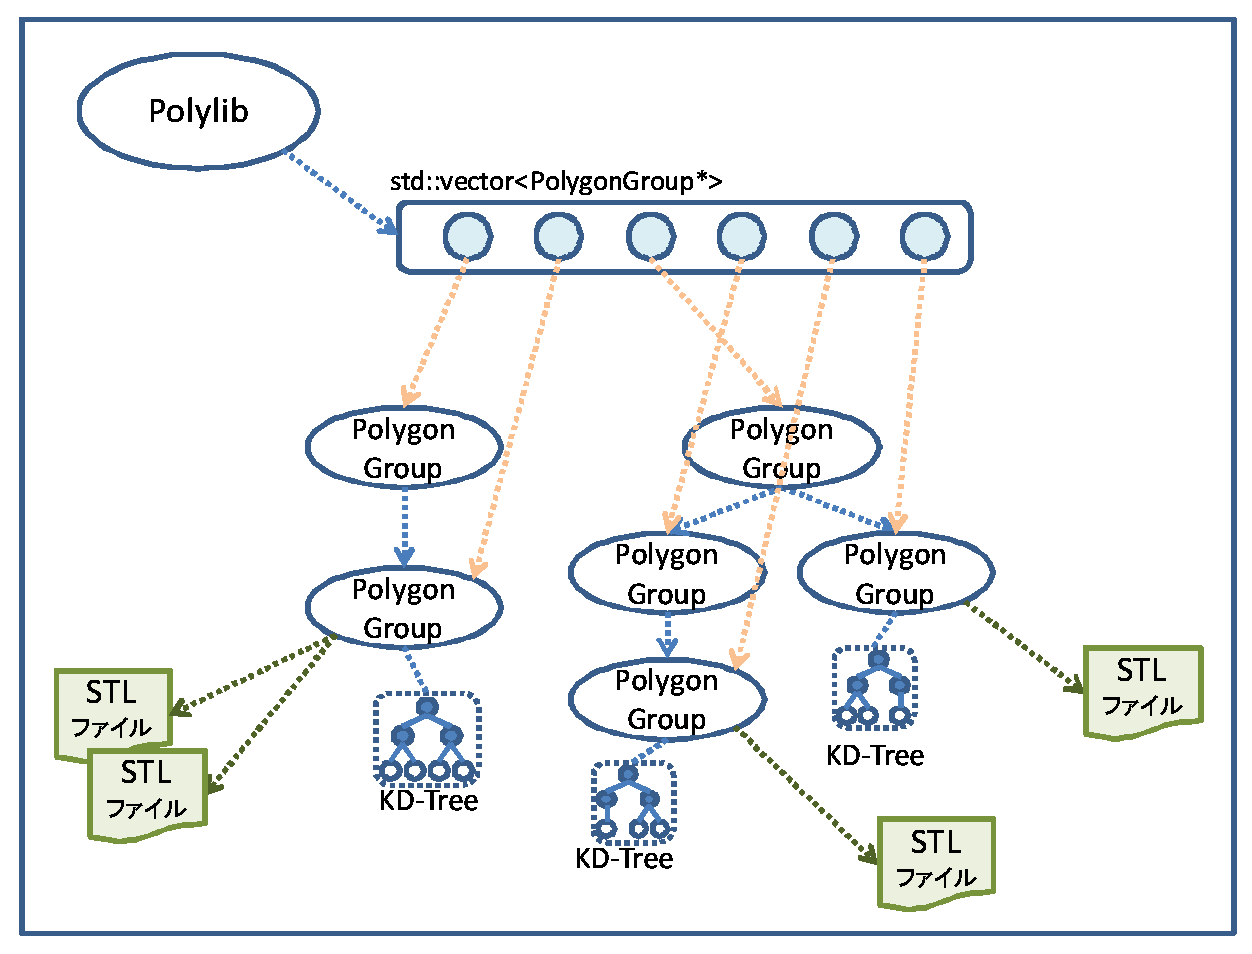
\includegraphics[width=10cm]{clip001.eps}
 \caption{ポリゴングループの管理構造}
\end{figure}

%
\subsection{ポリゴンデータの管理構造}

三角形ポリゴンの保持・管理は,Polygonsクラスのメンバ変数である,std::vector$<$PrivateTriangle*$>$ *m\_tri\_list
 で行います.このvectorコンテナには,STLファイルから読み込んだ三角形ポリゴン情報をPrivateTriangleクラス
インスタンスとして生成して登録します.

また,三角形ポリゴンを高速に検索するために,三角形ポリゴンのバウンディングボックスベースで包含判定を行う
KD-Tree構造を実装したTriMeshクラスをPolygonsクラスの導出クラスとして利用しています.KD木のリーフ要素で
ある三角形ポリゴン情報は,Polygons::m\_tri\_listコンテナに格納された各PrivateTriangleインスタンスへのポインタ
です.

Polylib::search()などのポリゴン検索メソッドは,このKD木を検索して得られたPrivateTriangle型ポインタの集合
をTriangle型ポインタにcastしてstd::vectorに詰めて返却します.検索メソッド呼び出し側では,返却結果の
std::vectorインスタンスを使用後にdeleteする必要がありますが,その要素であるTriangle型ポインタが指し示す
インスタンスを消去してはいけません.

\begin{figure}[H]
 \centering
 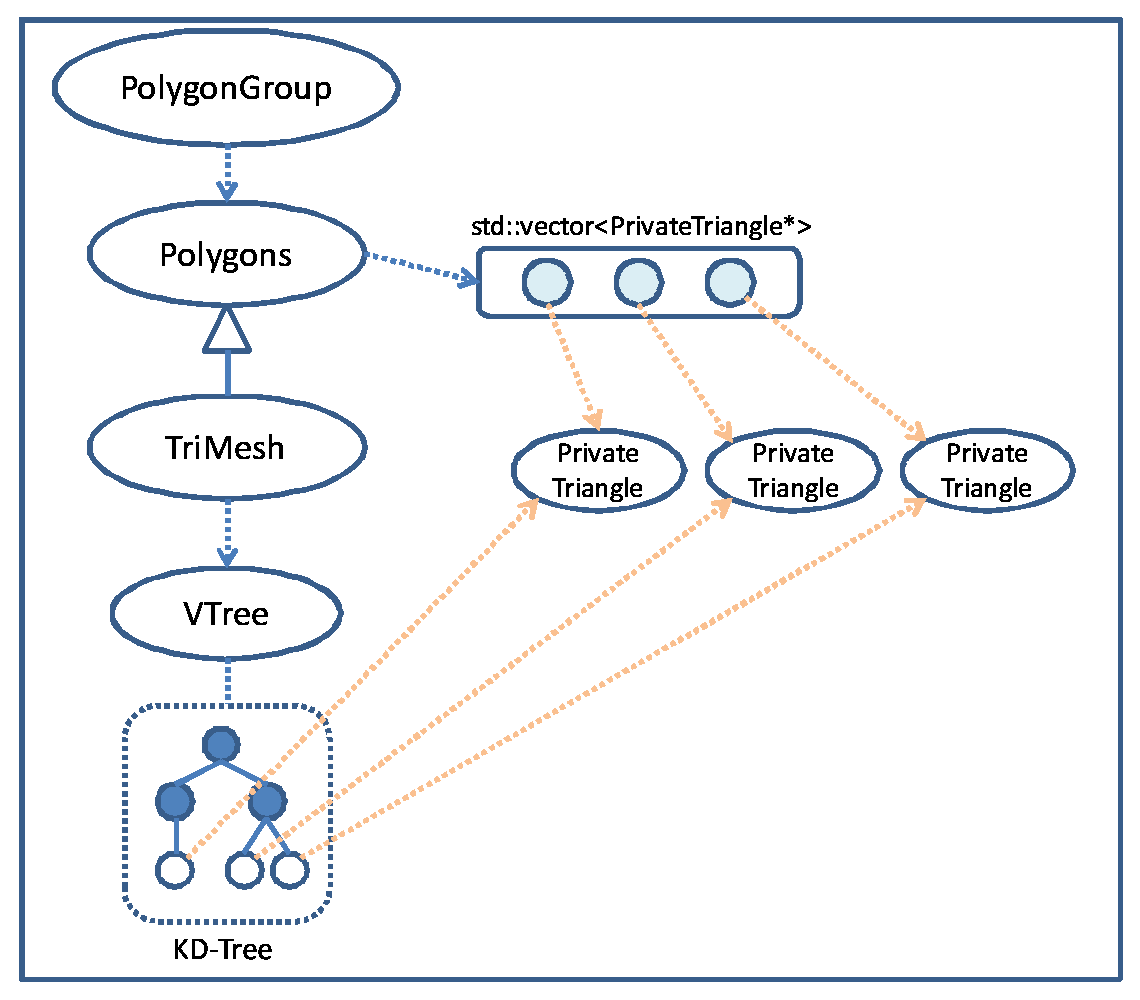
\includegraphics[width=8cm]{clip002.eps}
 \caption{ポリゴンデータの管理構造}
\end{figure}


%
\section{入力ファイル}

\subsection{Polylib初期化ファイル}

Polylib初期化ファイルは,Sphere初期化ファイルのユーザ定義パラメタ記述方式に準拠したXML形式のファイルです.
ElemタグとParamタグを利用して,ポリゴングループの階層構造を記述できます.ユーザ定義パラメタ記述方式の
基本的な考え方についてはSphereのマニュアルを参照してください.

Polylib初期化ファイルは,デフォルトではカレントディレクトリに存在する polylib\_config.xml を読み込みますが,
任意のファイル名をデータロードAPI引数で指定可能です.

記述例を以下に示します.

\begin{figure}[H]
 \centering
 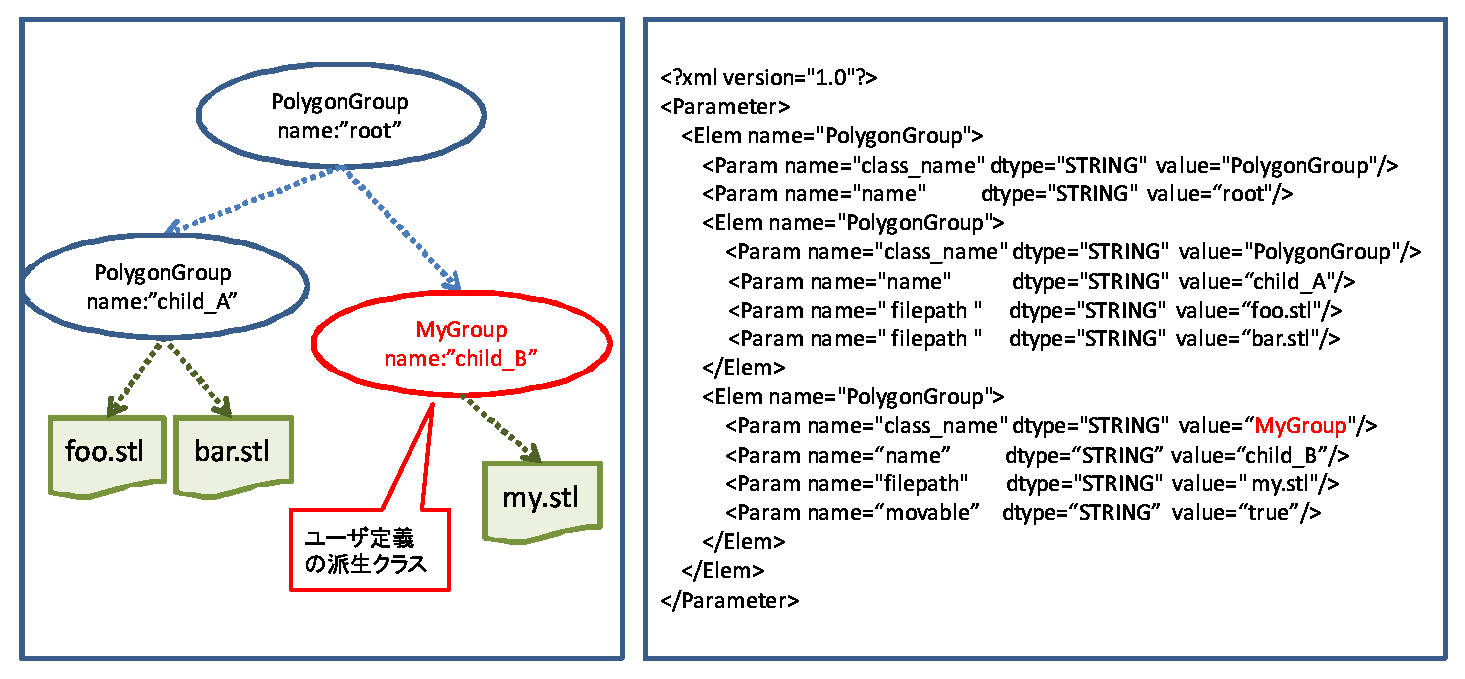
\includegraphics[width=16cm]{clip003.eps}\\
 \caption{初期化ファイルの例}
\end{figure}

各タグについて以下に説明します.

\begin{table}[htbp]
 \begin{tabular}{|l|p{34em}|} \hline
 タグ名 & 説明 \\\hline
 Parameter & Polylib初期化ファイルにおけるルートタグです.子要素としてElemタグを持つことができます. \\\hline
 Elem & ポリゴングループを表現します.子要素としてParamタグもしくはElemタグを持つことができます.name属性の値は必ず''PolygonGroup''でなければなりません. \\\hline
 Param & 各ポリゴングループの属性を表現します.子要素を持つことはできません. \\\hline
 \end{tabular}
 \caption{各タグの説明}
 \label{tbl:elem param}
\end{table}

\pagebreak

下表にParamタグの各属性値の書式を示します.

\begin{table}[htbp]
 \begin{tabular}{|l|l|p{34em}|} \hline
 name & dtype & 説明 \\\hline
 \hline
 class\_name & STRING & 生成するポリゴングループのクラス名.PolygonGroupクラスインスタンスを生成する場合は,''PolygonGroup''を指定.ユーザ定義の派生クラスインスタンスを生成する場合は,その派生クラスでオーバーライドしたメソッドget\_class\_name()が返す名称を指定する. \\\hline
 name & STRING & ポリゴングループの名称.名称は同じ階層内の同一レベルにおいて一意でなければならない. \\\hline
 \multicolumn{1}{|l|}{filepath} & \multicolumn{1}{l|}{STRING} & 当該ポリゴングループにひもづくSTLファイルのパス.カレントディレクトリからの相対パスまたは絶対パスで指定する. \\
 \multicolumn{1}{|l|}{} & \multicolumn{1}{l|}{} & 階層最下位のポリゴングループでのみ指定が可能. \\\hline
 \multicolumn{1}{|l|}{movable} & \multicolumn{1}{l|}{STRING} & 当該ポリゴングループがmove()メソッドにより移動するかどうかを指定する.valueには''ture''もしくは''false''を指定する. \\
 \multicolumn{1}{|l|}{} & \multicolumn{1}{l|}{} & 階層最下位のポリゴングループかつ,当該ポリゴングループがmove()メソッド実装済みのPolygonGroup派生クラスインスタンスの場合のみ指定が有効. \\\hline
 id & INT & ポリゴングループに付与可能なID番号.ID番号の重複は許される.省略可能で省略時は0が設定される.境界条件IDなどに利用されることを想定している. \\\hline
 \end{tabular}
 \caption{Paramタグの説明}
 \label{tbl:param tag}
\end{table}

上記Paramタグ属性値以外にも,ユーザ定義の属性値が指定可能です.ユーザ定義属性値の指定方法については,
後述のサンプルモデルによるチュートリアルを参照してください.

%
\subsection{STLファイル}
初期化ファイルで指定されたファイル名のSTLファイルを読み込みます.入力となるSTLファイルはアスキー形式
,バイナリ形式いずれでもかまいません.拡張子が"stl"であれば形式を自動判別して読み込みますが,拡張子が
"stla"であればアスキー形式として,"stlb"であればバイナリ形式として読み込みます.

%
\section{出力ファイル} \label{output_file}
本節では,Polylib::save()などのデータセーブ系APIで出力されたデータファイルについて説明します.

\subsection{Polylib初期化ファイル}

データセーブ時のポリゴングループの階層構造と,保存したSTLファイル名をpolylib初期化ファイル形式
で保存します.保存時のファイル命名規則は以下の通りです.

\begin{program}
	polylib_config_{ユーザ指定文字列}.xml
\end{program}

ユーザ指定文字列はデータセーブ系API引数で指定可能です.無指定の場合,保存時のタイムスタンプを
yyyymmddHHmmss形式で設定します.

%
\subsection{STLファイル}

データセーブ時のポリゴン情報を保存します.保存時のファイル命名規則は以下の通りです.

\begin{program}
	{ポリゴングループ名称フルパス}_{ユーザ指定文字列}.{stla|stlb}
\end{program}

ポリゴングループ名称フルパスとは,階層最上位のポリゴングループ名称から,当該グループ名称までを
'\_'でつなげたものです.
ユーザ指定文字列はデータセーブ系API引数で指定可能です.無指定の場合,保存時のタイムスタンプを
yyyymmddHHmmss形式で設定します.

ファイル拡張子はデータセーブ系APIで指定した保存ファイル形式に基づき設定されます.

MPIPolylibの場合,当該ポリゴングループについて自ランク内に保存すべき三角形ポリゴン情報が存在
しない場合はSTLファイルは出力されません.

なお,データロード時に指定したpolylib初期化ファイルにおいて,複数のSTLファイルを指定したポリゴン
グループについてデータセーブを行うと,ポリゴン情報は1つのSTLファイルに纏めて出力されます.

%
\subsection{三角形IDファイル}

MPIPolylib::save\_parallel()を利用したデータセーブ時にSTLファイル内の三角形ポリゴン並びに対応した三角形IDを保存します.

三角形IDとはMPIPolylibが管理する全三角形ポリゴン情報に対し,その三角形が所属するポリゴングループ内
で一意となるようなint型のID番号で,MPIPolylib内部でデータロード時に自動的に付与されます.

並列動作時に各ランク毎にデータセーブする場合,各計算領域ガイドセル部分の三角形情報は重複して保存
されるため,データを再ロードした際に重複三角形を判別するために三角形ID情報ファイルが必要となりま
す.

保存時のファイル命名規則は以下の通りです.

\begin{program}
	{ポリゴングループ名称フルパス}_{ユーザ指定文字列}.id
\end{program}

ポリゴングループ名称フルパスとは,階層最上位のポリゴングループ名称から,当該グループ名称まで
を'\_'でつなげたものです.

ユーザ指定文字列はデータセーブ系API引数で指定可能です.無指定の場合,保存時のタイムスタンプを
yyyymmddHHmmss形式で設定します.

なお,当該ポリゴングループについて自ランク内に保存すべき三角形ポリゴン情報が存在しない場合は三角形IDファイルは出力されません.
